%
% 総合研究概要書原稿サンプルファイル
%
% ・題名, 英文題名, 研究室名, 学籍番号, 氏名, 指導教員名 は1段組,
%   本文は2段組.全体で2ページ。ページ番号は不要。
% ・カラー使用可だが,PDF化したときにファイルサイズが最大 5MB 程度に収まるようにすること。
% ・ファイル名は半角英数字で「学籍番号氏名_●●研.pdf(●●は指導教員の姓,例:BV18000数理科太郎_福田研.pdf)」とする。
% ・余白, フォントサイズなどは多少変えてもよいが, あまり大幅に
%   変更しないように.他の人の概要とのバランスも考えて.
%
\documentclass[twocolumn]{jarticle}
\usepackage{amsmath,amsfonts,amssymb}
\usepackage{color}
\usepackage[dvipdfm]{graphicx}
\usepackage{booktabs}
\usepackage{here}

%定理環境の設定
\usepackage{amsthm}
\theoremstyle{definition}
\newtheorem{theorem}{定理}[section]
\newtheorem{definition}[theorem]{定義}
\newtheorem{lemma}[theorem]{補題}
\newtheorem{axiom}[theorem]{公理}
\newtheorem{proposition}[theorem]{命題}
\newtheorem{corollary}[theorem]{系}
\newtheorem{example}[theorem]{例}
\newtheorem*{theorem*}{定理}
\newtheorem*{definition*}{定義}
\newtheorem*{lemma*}{補題}
\newtheorem*{axiom*}{公理}
\newtheorem*{proposition*}{命題}
\newtheorem*{corollary*}{系}
\newtheorem*{example*}{例}
\renewcommand\proofname{\bf 証明}

\pagestyle{empty}
\setlength\textheight{255mm}
\setlength\textwidth{170mm}
\setlength\topmargin{-5mm}
\setlength\oddsidemargin{-5mm}
\setlength\headheight{0mm}
\setlength\headsep{0mm}
\setlength\columnsep{8mm}
%**************************
\title{
  \LARGE\bf
  多様体の次元を調べる方法 \\[1ex]
  \Large\bf
  Methods for Investigating the Dimension of Manifolds}
\author{空間数理研究室 \quad
        BV20052 青見 健志 \quad
        指導教員 亀子 正喜 教授}
\date{}
%**************************
\begin{document}
\maketitle
\thispagestyle{empty}

\section{はじめに}
どこでも好きなところに$m$次元の局所座標系
を描ける空間を$m$次元多様体という. 例えば, 球面
は球面上のどこでも好きなところに
$2$次元の局所座標系を描くことができるため, 
$2$次元多様体である.  

私は複雑な方程式で表された空間や
高次元の空間などの形を理解することに興味をもち, 
多様体の次元を調べる方法を研究することにした. 
\begin{figure}[H]
    \centering
    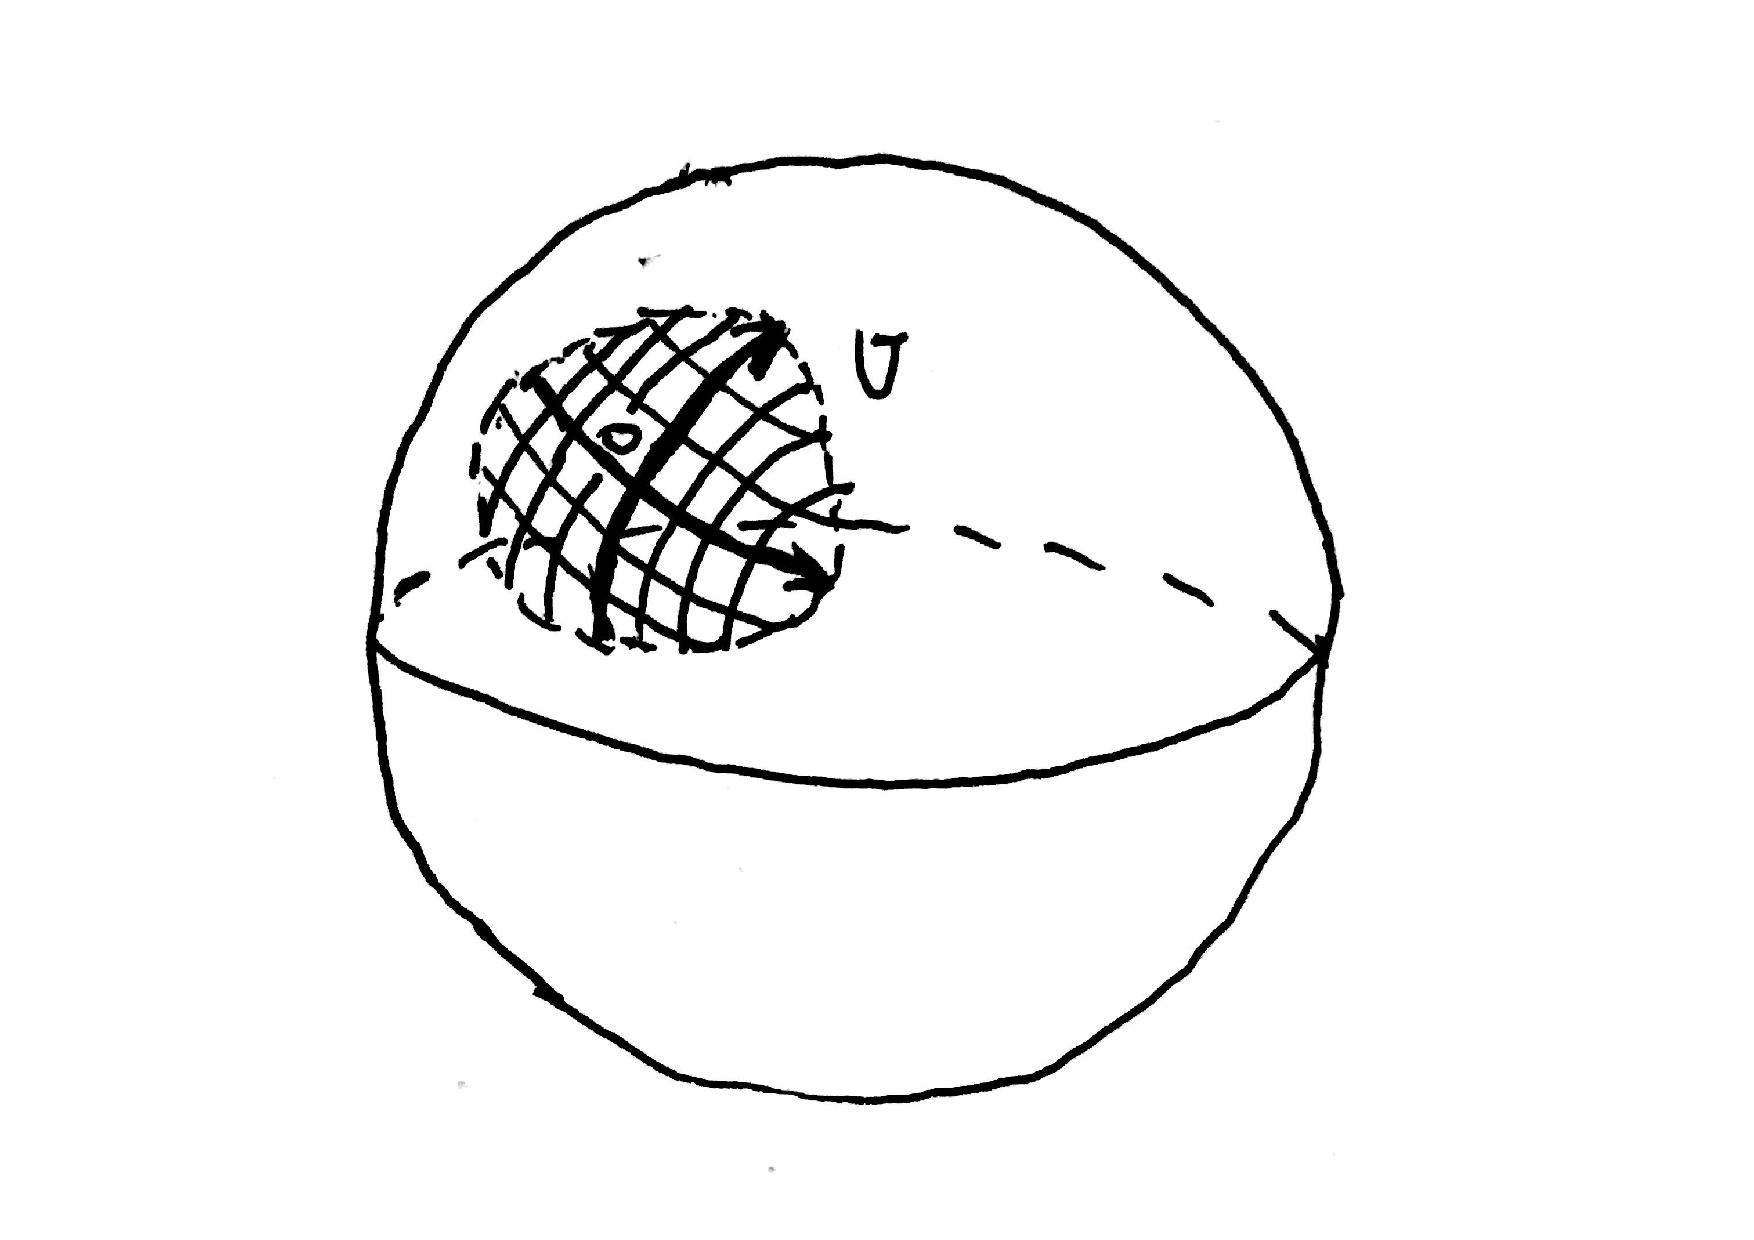
\includegraphics[keepaspectratio, scale=0.15]
         {CoSysInS2.pdf}
    \caption{球面に描かれた局所座標系}
    \label{CoSysInS2}
   \end{figure}

\section{数式の例}
\begin{definition}\label{def:C^r manifold}
  $r\geq 1$を自然数または$\infty$とする. 
  位相空間$M$が次の条件(1), (2), (3)を満たすとき, 
  $M$を$m$次元$C^r$級多様体という.
  \begin{itemize}
      \item[(1)]$M$はハウスドルフ空間である.
      \item[(2)]$M$は$m$次元座標近傍により被覆される. 
      すなわち, $M$の$m$次元座標近傍からなる族
      $\{(U_\alpha, \varphi_\alpha)\}_{\alpha \in A}$
      があって, 
      $$M = \bigcup_{\alpha \in A}U_\alpha$$
      が成り立つ. 
      \item[(3)]$U_\alpha \cap U_\beta \neq \phi$
      であるような任意の$\alpha$, $\beta$に対して, 座標変換
      $$\psi \circ \varphi:\varphi(U\cap V)\rightarrow \psi(U\cap V)$$
      は$C^r$級写像である. 
  \end{itemize}
\end{definition}
\begin{theorem}
  $m$次元球面$S^m \in \mathbb{R}^{m+1}$を
  $$S^m=\{(x_1,\cdots x_{m+1})|x_1^2+\cdots +x_{m+1}^2=1\}$$
  と定義すると, $S^m$は$m$次元$C^{\infty}$級多様体である. 
\end{theorem}
\begin{proof}
  $\mathbb{R}^{m+1}$はハウスドルフ空間
      であるから, その部分空間として, $S^m$は
      ハウスドルフ空間である. 
      $S^m$の$2(m+1)$個の開集合
      $U_i^+$, $U_i^-$ $(i=1,\cdots ,m+1)$を
      次のように定義する. 
      $$U_i^+ = \{(x_1, \cdots x_i, \cdots ,x_{m+1})\in S^m|x_i>0\}$$
      $$U_i^- = \{(x_1, \cdots x_i, \cdots ,x_{m+1})\in S^m|x_i<0\}$$
      $S^m$はこれら$U_i^+$, $U_i^-$ $(i=1,\cdots ,m+1)$
      で被覆される. 写像$\varphi_i^+:U_i^+ \rightarrow \mathbb{R}^m$, 
      $\varphi_i^-:U_i^- \rightarrow \mathbb{R}^m$を
      それぞれ次のように定義する. 
      $$\varphi_i^+(x_1,\cdots ,x_i,\cdots, x_{m+1})=(x_1,\cdots ,\hat{x_i},\cdots ,x_{m+1})$$
      $$\varphi_i^-(x_1,\cdots ,x_i,\cdots, x_{m+1})=(x_1,\cdots ,\hat{x_i},\cdots ,x_{m+1})$$
      ここで, $\hat{x_i}$は$x_i$を取り去るという意味である. このとき, 
      $\varphi_i^+$, $\varphi_i^-$はそれぞれ, $U_i^+$, 
      $U_i^-$から$\mathbb{R}^m$への射影であるから, 同相写像であり, 
      すべての座標変換$\varphi_b^+\circ(\varphi_a^+)^{-1}\ 
      (1\leq a, b\leq 2(m+1))$が$C^{\infty}$級であることが確かめられる. 
      よって, $S^m$は$m$次元$C^{\infty}$級多様体であることがわかる. 
\end{proof}
\begin{figure}[H]
  \begin{tabular}{cc}
    %---- 最初の図 ---------------------------
    \begin{minipage}[t]{0.45\hsize}
      \centering
      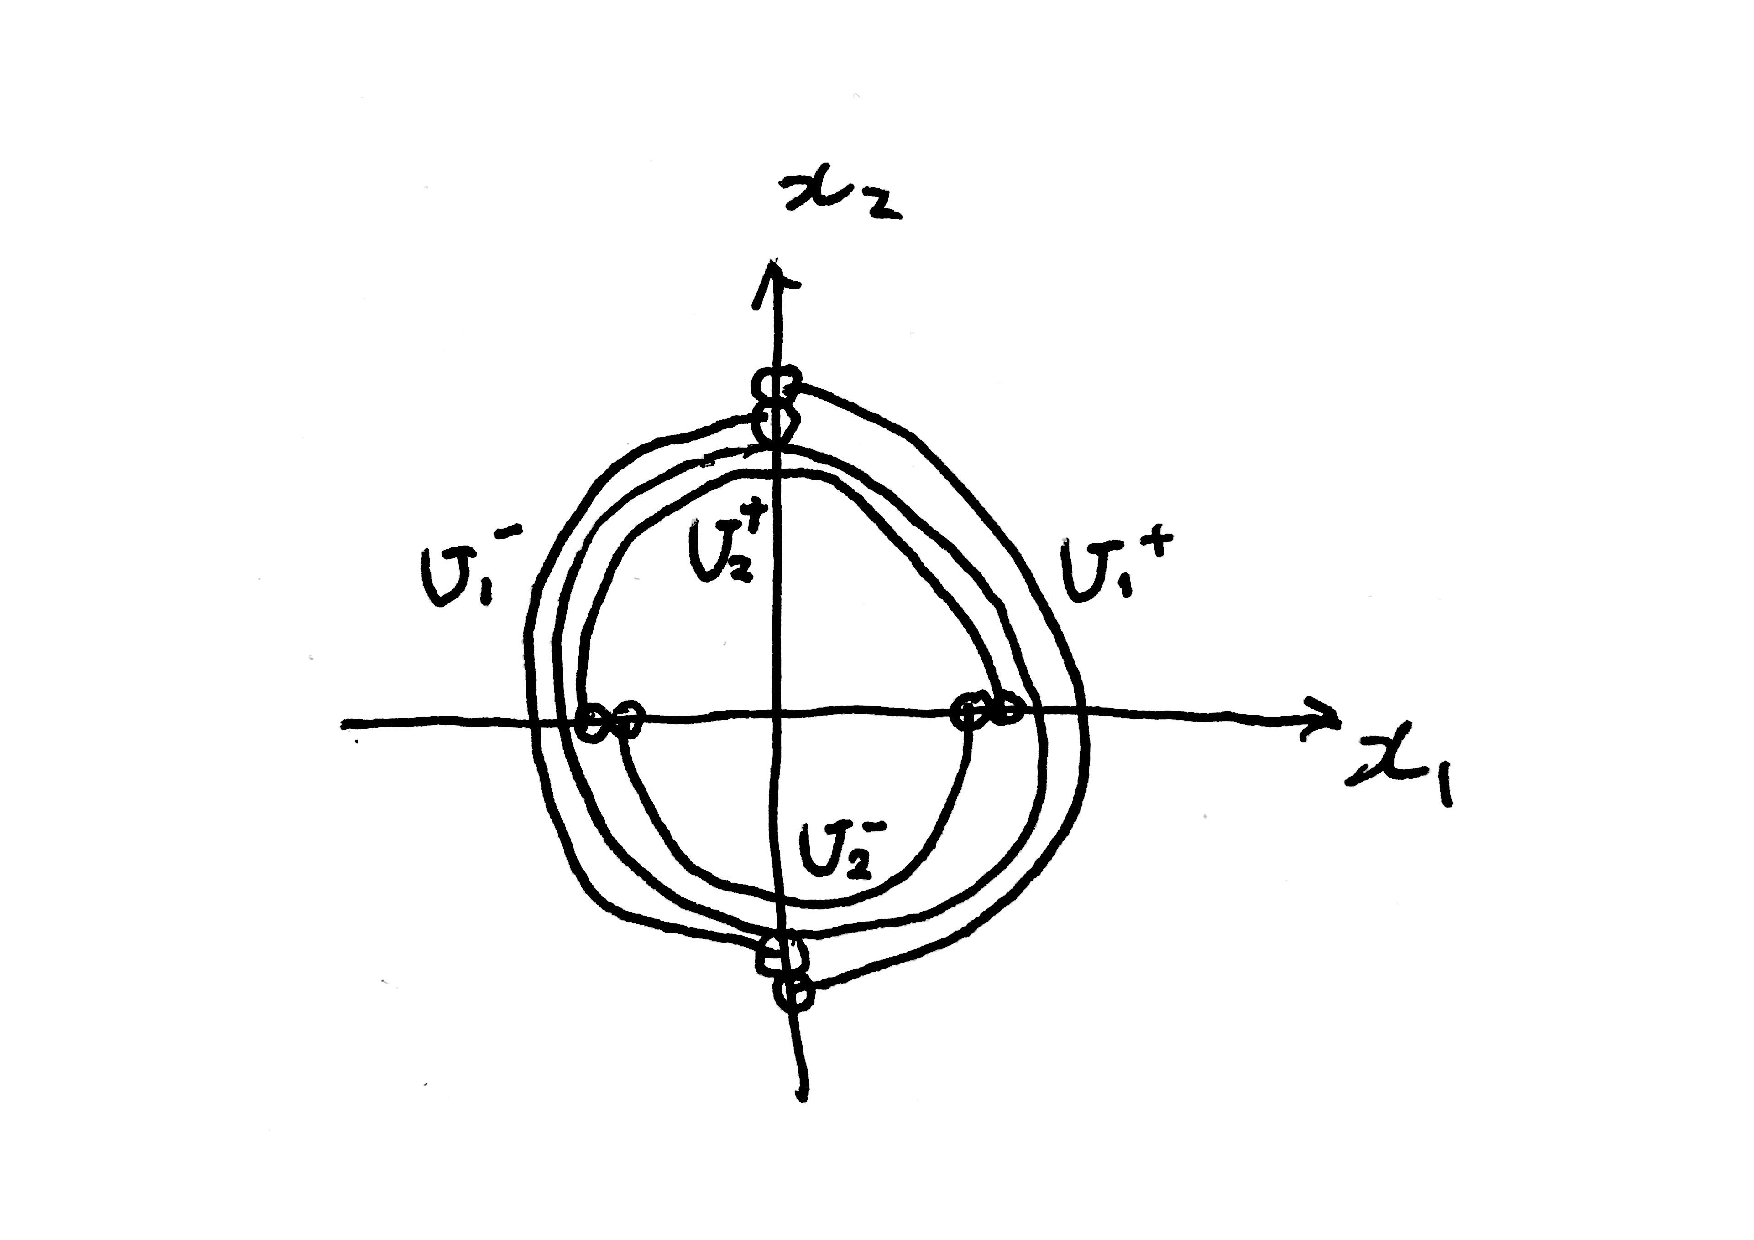
\includegraphics[keepaspectratio, scale=0.2]{localCoSysOfS1_1.pdf}
      \caption{$S^1$の開集合}
      \label{}
    \end{minipage} &
    %---- 2番目の図 --------------------------
    \begin{minipage}[t]{0.45\hsize}
      \centering
      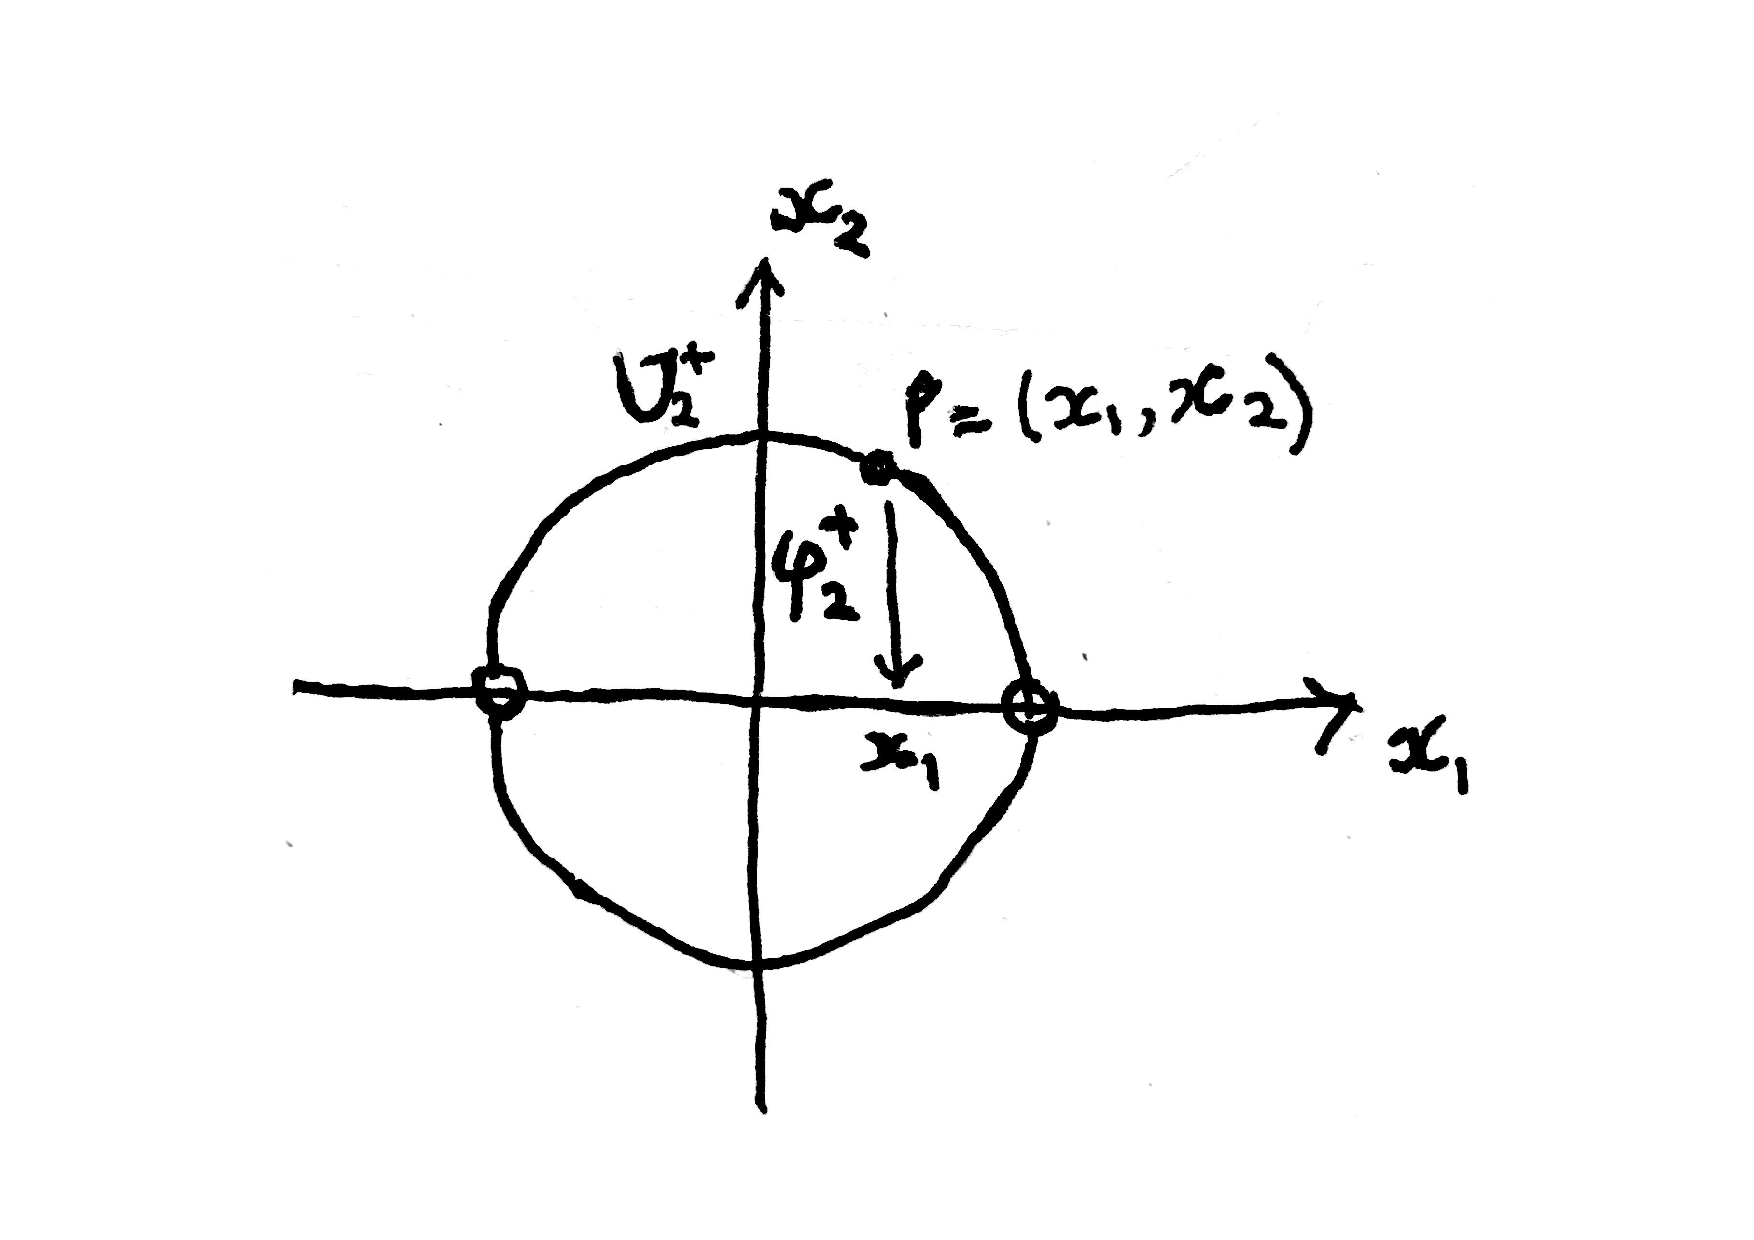
\includegraphics[keepaspectratio, scale=0.2]{localCoSysOfS1_2.pdf}
      \caption{$S^1$の局所座標系}
      \label{}
    \end{minipage}
    %---- 図はここまで ----------------------
  \end{tabular}
\end{figure}

\begin{definition}\label{def:C^s deffeomorphism}
  $M$, $N$を$C^r$級多様体とする. $f:M\to N$
  が$C^s$級微分同相写像であるとは, 次の条件
  (1), (2)を満たすことをいう. 
  \begin{itemize}
      \item[(1)]
      $f:M\to N$は全単射($1$対$1$かつ上への写像)
      である. 
      \item[(2)] 
      $f:M\to N$と$f^{-1}:N\to M$はともに$C^s$
      級写像である. 
  \end{itemize}
  ここで$f:M\to N$が$C^s$級写像であるとは, 
  $p\in M$, $f(p)\in N$を含む$C^r$級
座標近傍$(U,\varphi)$, $(V,\psi)$に対して
  $\psi^{-1} \circ f\circ \varphi$が
  $C^s$級写像であるということである. 
\end{definition}
\begin{definition}
  $p$を含む座標近傍$(U;x_1,\cdots x_m)$を
  $1$つ固定する. $p$のまわりで定義された
  $C^r$級関数$f$に, $p$における$x_i$
  方向の偏微分係数を対応させる操作を
  $\left(\frac{\partial}{\partial x_i}
  \right)_p$と書く. すなわち, 
  $$\left(\frac{\partial}{\partial x_i}
  \right)_p:f\mapsto 
  \frac{\partial f}{\partial x_i}(p)$$
  である. 
\end{definition}
\begin{proposition} 
  $m$個のベクトル
  $\left(\frac{\partial}{\partial x_1}\right)_p, 
  \cdots 
  \left(\frac{\partial}{\partial x_m}\right)_p$
  は$1$次独立である. 
\end{proposition}
\begin{definition}\label{def:tangent vector space}
  $m$個のベクトル
  $\left(\frac{\partial}{\partial x_1}\right)_p, 
  \cdots 
  \left(\frac{\partial}{\partial x_m}\right)_p$
  の張るベクトル空間を, 点$p$
  における$M$の接ベクトル空間とよび, 
  $T_p(M)$
  という記号で表す. 接ベクトル空間$T_p(M)$の
  元を接ベクトルとよぶ. 
\end{definition}
\begin{figure}[H]
      \centering
      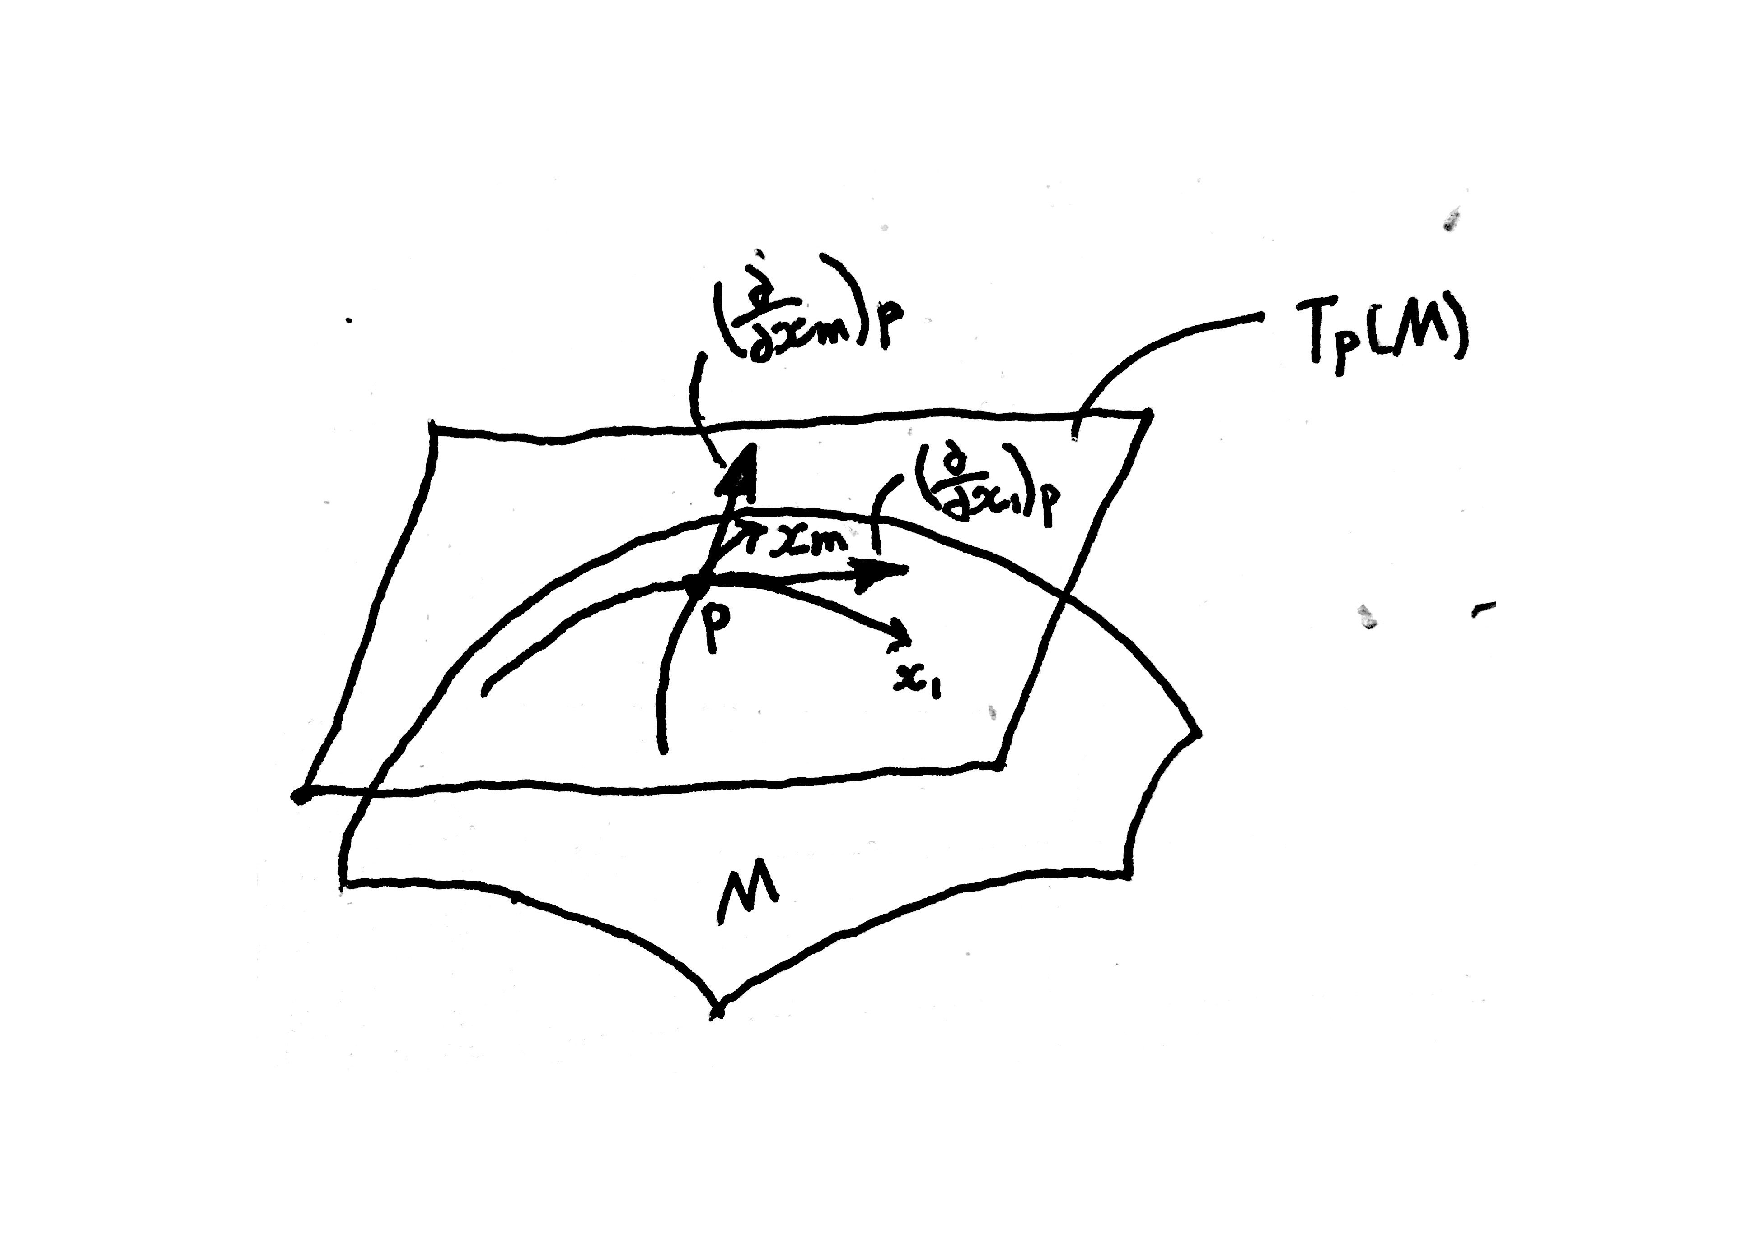
\includegraphics[keepaspectratio, scale=0.3]{tangentVectorSpace_2.pdf}
      \caption{$T_p(M)$のイメージ}
      \label{}
\end{figure}
$T_p(M)$は点$p$のまわりの局所座標系のとり方に
よらず一意に定まる. 
\begin{proposition}\label{prop:relation of v and w}
  $t=0$におけるj曲線$c$, $f\circ c$の速度ベクトルを
  それぞれ
  $$\left .\frac{dc}{dt}\right|_{t=0}=
  \sum_{i=1}^{m}v_i\left(\frac{\partial}
  {\partial x_i}\right)_p,\ 
  \left .\frac{d(f\circ c)}{dt}\right|_{t=0}=
  \sum_{j=1}^{n}w_j\left(\frac{\partial}
  {\partial y_j}\right)_q$$
  とおくと, 係数$v_1,\cdots ,v_m$と
  $w_1,\cdots ,w_n$の間には次の関係がある. 
  $$w_j=\sum_{i=1}^{m}\frac{\partial f_j}
  {\partial x_i}(p)v_i\ (j=1,\cdots ,n)$$
  またこの式を, 縦ベクトルと行列を使って書くと
  $$\begin{pmatrix}
        w_1 \\
        \vdots \\
        w_n 
      \end{pmatrix}
      =
      \left(
      \begin{array}{ccc}
        \frac{\partial f_1}{\partial x_1}(p)&\cdots &\frac{\partial f_1}{\partial x_m}(p)\\
        \vdots &\ddots& \vdots \\
        \frac{\partial f_n}{\partial x_1}(p)&\cdots &\frac{\partial f_n}{\partial x_m}(p) 
      \end{array} 
      \right)
      \begin{pmatrix}
        v_1\\
        \vdots \\
        v_m
      \end{pmatrix}
      $$
  となる. 上の$n$行$m$列の行列を点$p$における
  ヤコビ行列とよび, $(Jf)_p$で表す. 
\end{proposition}
\begin{definition}\label{def:differential}
  $$(df)_p:T_p(M)\to T_{f(p)}(N),\ 
  \begin{pmatrix}
    v_1\\
    \vdots \\
    v_m
  \end{pmatrix}
  \mapsto
  (Jf)_p
  \begin{pmatrix}
    v_1\\
    \vdots \\
    v_m
  \end{pmatrix}$$
  を, 点$p$における$f:M\to N$
  の微分とよぶ. 
\end{definition}
\begin{theorem}\label{theo:f^{-1}(q) C^r manifold}
  $M$, $N$を$m$次元, $n$次元の$C^r$級多様体, 
  $f:M\to N$を$C^r$級写像とする. $N$のある点
  $q$について, $f(p)=q$となる$M$の各点$p$
  が常にrank$(Jf)_p=n$を満たすとき, 逆像
  $f^{-1}(q)$は$(m-n)$次元$C^r$級多様体
  である. 
\end{theorem}

\begin{example}
  $2$次元トーラス$T^2=S^1\times S^1$は
  $2$次元$C^\infty$級多様体になる. 

  $T^2=\{(x_1,x_2,x_3,x_4)\in \mathbb{R}^4|
  x_1^2+x_2^2=1, x_3^2+x_4^2=1\}$
  より, 
  $C^\infty$級写像$f:\mathbb{R}^4\to \mathbb{R}^2$
  を$f(x_1,x_2,x_3,x_4)=(x_1^2+x_2^2-1,
  x_3^2+x_4^2-1)$と定義すると, 
  $T^2=f^{-1}(0,0)$
  と表せる. ヤコビ行列$(Jf)_{\boldsymbol{x}}$は
  $$(Jf)_{\boldsymbol{x}}=
      \left(\begin{array}{cccc}
          2x_1&2x_2&0&0\\
          0&0&2x_3&2x_4
      \end{array}\right)$$
  $\boldsymbol{x}\in T^2$のとき, 
  rank$(Jf)_{\boldsymbol{x}}=2$であるから, 
  $T^2$は$4-2=2$次元$C^\infty$級
  多様体である. 
\end{example}
%参考文献
\begin{thebibliography}{99}
  \bibitem{Matsumoto18} 松本幸夫, [第30版]多様体の基礎, 東京大学出版会, 2018.
  \bibitem{Hujioka17} 藤岡敦, [第2版]具体例から学ぶ 多様体, 裳華房, 2017.
  \bibitem{Hattori76} 服部晶夫, [第1版]多様体, 岩波書店, 1976.
  %\bibitem{b}【論文の場合】著者名,タイトル,雑誌名,巻・号,出版年度,頁.
  %\bibitem{c}【Webページの場合】 タイトル,ページ制作者(機関)等,URL: \url{http://www.shibaura-it.ac.jp/},最終アクセス日時: 2021/12/28 16:33.
  \end{thebibliography}
\end{document}  	  

